% As for 2D OSG, it is similar to the metric k-center problem and therefore
% the approximation algorithms solving k-center problem can be applied to 2D OSG. 

In their general forms, Problems~\ref{p:surf-1}-\ref{p:surf-3} require the computation of 3D visibility, a hard task on its own. Due to this reason, a polynomial time algorithm with guaranteed good approximation ratio for these problems appear difficult to come by. It is an interesting question to ask whether some form of approximation scheme can be derived. Here, we show that for Problem~\ref{p:surf-2}, if one relax the visibility requirement, i.e. letting $vis(\cdot, \cdot)\equiv 1$, then a polynomial time $(2+\varepsilon)$-approximation algorithm can be obtained. 

Taking Problem~\ref{p:surf-2}, we examine a setup assuming that each point $p \in S$ has good visibility, i.e., $p$ is always visible to the nearest sensor. Such scenarios happen when the 3D domain does not have large curvatures that would easily block sensors' view, e.g., covering the earth with GPS satellites or using drones to survey a vineyard. To drive a specific approximation bound, 
we further assume that sensors have spherical range sensing and are in a plane of some fixed height $h$ from the ground, which may be relaxed. 
\begin{wrapfigure}{r}{1.5in}
  % \vspace*{0mm}
  % \begin{overpic}[width=1.3in,tics=5]
  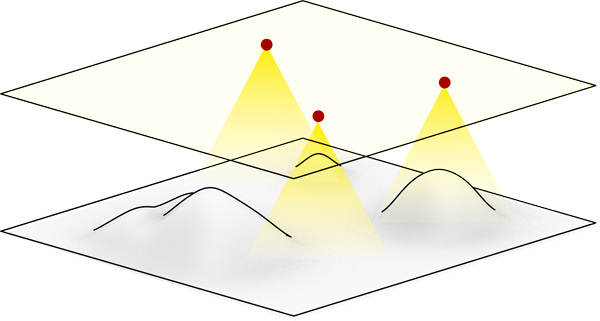
\includegraphics[width=1.5in]{chapters/surf/fig/env.png}
	% \end{overpic}
  % \vspace*{-6.5mm}
\end{wrapfigure}
Denote this surface as $H_C$. 
The figure on the right provides an illustration of the target environment setting. 

The main idea is to first obtain a dense sample of $S$ and then adapt $2$-approximation algorithms for the corresponding 2D setting, which requires some non-trivial reasoning. Two well-known approximation algorithms for $k$-center like problem in 2D are based on \emph{farthest point clustering} \cite{gonzalez1985clustering} and \emph{dominating set} \cite{hochbaum1985best, vazirani2013approximation}. Both of these approaches work for our purpose; we show how to work with the former.

Let a uniformly sampled set of points of $S$ be $S_N = \{o_1, \ldots, o_N\}$. We apply the farthest point clustering \cite{gonzalez1985clustering} on $S_N$ as follows. As the name suggest, it picks farthest sensor locations until the number of sensors are exhausted. In the original approach, the points to be clustered are also sensor locations, which is not true here. Instead, we perform clustering in the set $S_N$ and project the selected samples to $H_C$ gradually. The relatively straightforward process is given in Algorithm~\ref{alg:surf-greedy} (($d(\cdot$,$\ \cdot)$ denotes the distance between the inputs, one or both of which may be sets).


\begin{algorithm}
\begin{small}
    \SetKwInOut{Input}{Input}
    \SetKwInOut{Output}{Output}
    \SetKwComment{Comment}{\% }{}
    \caption{Farthest Point Clustering}
		\label{alg:surf-greedy}
    \SetAlgoLined
		\vspace{1mm}
    \Input{$S_N$=\{$o_1, \dots, o_N$\}: $N$ sampled points on the surface $S\subset \partial \mathcal E$; $k$: number of sensors;\\
    $H_C$: a plane with a fixed height}
    \Output{$\mathcal{C}$: sensor location set}
		\vspace{1mm}
        % $\mathcal C$ = $\varnothing$\\
        $\mathcal{C} \leftarrow$  \{$o_1$'s vertical projection onto $H_C$\}\\
        % \While{$|\mathcal{C}|<k$}{
        \For{$i \gets 1$ \KwTo $k$}{
        \For{$o\in S_N$}{
        compute the distance $d(o, \mathcal{C})$ between $o$ and $\mathcal{C}$\\ 
        }
        $o \leftarrow$ point $v\in S_N$ with the largest $d(v,\mathcal{C})$\\
        $\mathcal{C} \leftarrow \mathcal{C}\ \cup \{o$'s projection onto $H_C$\}\\
        % $p^\star \leftarrow$ the projection of $v^\star$ on height $H$\\
        % Add $p^\star$ to $\mathcal{C}$\\
        }
        \Return $\mathcal{C}$
\end{small}
\end{algorithm}

To prove the claimed $(2+\varepsilon)$-approximation bound,  
denote the optimal sensor location set and the sensor location set derived by Algorithm~\ref{alg:surf-greedy} as $\mathcal{C}_{OPT}$ and $\mathcal{C}$, respectively. Since these are centers of spherical sensing ranges, we call them center set for short. Denote the minimum coverage radius in the spherical sensing model as $r_{OPT}$. Let $h$ be the minimum distance between surface $S$ and sensor space $H_C$, i.e. $h:=d(S,H_C)$. $r_{OPT}$ and $r_{\mathcal{C}}$ are defined as follows:
\begin{equation}
    r_{OPT}:=\max_{o\in S_N} d(o, \mathcal{C}_{OPT})
\end{equation}
\begin{equation}
    r_{\mathcal{C}}:=\max_{o\in S_N} d(o, \mathcal{\mathcal{C}})
\end{equation}

\begin{proposition}
\label{prop:surf-algo1t}
The center set obtained by Algorithm~\ref{alg:surf-greedy} achieves coverage radius of at most
%$r_{OPT} + \sqrt{r_{OPT}^2 - h^2}$
$\sqrt{4r_{OPT}^2 - 3h^2}$.
\vspace{-1mm}
\end{proposition}
\begin{proof}

%So we need to prove:
%\begin{equation}
%    r^{C}\leq 2r^{OPT}
%\end{equation}

Denote the center set generated at the 
$i$th round as $\mathcal{C}_{i}$, and $r_i$ as the cluster radius $r_i := \max_{o_\tau}\min_{c_j \in \mathcal{C}_i} d(o_\tau, c_j)$. It is straightforward to observe that $r_k\leq r_{k-1} \leq \dots \leq r_1$.
Consider the relationship between the optimal center set $\mathcal{C}_{OPT}$ and the center set obtained by Algorithm~\ref{alg:surf-greedy}, we have the following 2 cases.

Case 1: For each sphere $\mathcal{B}_{c}$ centered at a point $c\in\mathcal{C}_{OPT}$ with radius of $r_{OPT}$, the projection of $\mathcal{B}_{c}\bigcap S$ onto the sensor space $H_C$
contains exactly one point of $\mathcal{C}_k$. 

% \kg{KG: Since we have a projection step, the OPT sphere needs to cover not only the center, but also the points that project to the center}

In this case, let $v$ be an arbitrary point in $S$. 
Let $c_{\alpha}$ be the nearest center to $v$ in $\mathcal{C}_{OPT}$ 
and $c_{\beta}$ be the point in $\mathcal{C}_k$ whose projection on $S$ is inside $\mathcal{B}_{c_{\alpha}}$. 
Therefore, we have: 
\begin{equation}
    d(v, c_\beta) 
    % \leq d(v,c_{\alpha}) + d(c_{\alpha}, c_\beta) 
    \leq 
    %r_{OPT} + \sqrt{r_{OPT}^2-h^2}
    \sqrt{4r_{OPT}^2 - 3h^2}
\end{equation}

Case 2: There exists a sphere $\mathcal{B}_{c}$ centered at a point $c\in\mathcal{C}_{OPT}$ with radius of $r_{OPT}$, the projection of $\mathcal{B}_{c}\bigcap S$ onto the sensor space $H_C$
contains at least 2 points of $\mathcal{C}_k$. 
In this case, denote the two centers by $c_i$ and $c_j$ $(i<j)$, and their projections on $S$ are in the same sphere $\mathcal{B}_c$. As $c_j$ is added after $c_i$, then,
%Without loss of generality, we can assume that $c_2$ is added in the $i^{th}$ iteration and is no less than $c_1$.% then we have:
\begin{equation}
    \begin{split}
    r_\mathcal{C} = r_k 
    &\leq r_{j}
    \leq d(c_i, c_j\text{'s projection on } S)\\
    &\leq \sqrt{4r_{OPT}^2 - 3h^2}
    % \\
    % &\leq \sqrt{r_{OPT}^2 - h^2} + r_{OPT}\\
    \end{split}
\end{equation}
Summarizing the two cases proves Proposition~\ref{prop:surf-algo1t}.
\vspace{-2mm}
\end{proof}

% \begin{remark}
% With a finer analysis, it can be shown both approximation algorithms are guaranteed to produce at most $\sqrt{4r_{OPT}^2 - 3h^2}$ spherical radius.
% \end{remark}
\vspace{-0.05in}